\section{Introduction}
\label{sec:intro}

%% WHAT IS AD HOC DATA?

An {\em ad hoc data format} is any non-standard data format for which
parsing, querying, analysis, or transformation tools are not readily
available.  Despite the increasing use of standard data formats such
as \xml{}, ad hoc data sources continue to arise in numerous
industries such as finance, health care, transportation, and
telecommunications as well as in scientific domains, such as
computational biology and chemistry.  The absence of tools for
processing ad hoc data formats complicates the daily data-management
tasks of data analysts, who may have to cope with numerous ad
hoc formats even within a single application.  

Common characteristics of ad hoc data complicate the building of tools
to perform even basic data-processing tasks.  Documentation of ad hoc
formats, for example, is often incomplete or inaccurate, making it
difficult to define a database schema for the data or to build a
reliable data parser.  The data itself often contains numerous kinds
of errors, which can thwart standard database loaders.  Surprisingly,
few meta-language tools, such as data-description languages or parser
generators, exist to assist in management of ad hoc data.  And
although ad hoc data sources are among the richest for database and
data mining researchers, they often ignore such sources as the work
necessary to clean and vet the data is prohibitively expensive.

\cut{Before the data can be processed
reliably by an application, errors must be identified, filtered out,
or corrected, and the cleansed data must be transformed into a
standard loading format.
such as loading ad hoc data into a database system. 

Once in a standardized format, the data can be directly loaded into a
database or manipulated by standard, widely available tools.}

%% EXAMPLE SOURCES AND CHARACTERISTICS

\cut{\xml{}, for
example, is not ad hoc, because numerous, standard tools for parsing,
querying, and transforming exist for \xml{}.
There are vast amounts of useful data stored in traditional databases
and \xml{} formats, but there is just as much in ad hoc formats.}

The variety of application domains, format characteristics, sources of
errors, and volume of data makes processing ad hoc data both
interesting and challenging.  \figref{figure:data-sources} summarizes
several ad hoc sources from the networking and telecommunication
domains at AT\&T and from computational biology applications at
Princeton.  Formats include ASCII, binary, and Cobol, with both fixed
and variable-width records arranged in linear sequences and in
tree-shaped or DAG-shaped hierarchies.  Even within one format, there
can be a great deal of syntactic variability.  For example,
\figref{fig:darkstar-records1} contains two records from the
network-monitoring application.  Note that each record has different
number of fields (delimited by '$|$') and that individual fields contain
structured values (e.g., attribute-value pairs separated by '=' and
delimited by ';').

%% WHY IS PROCESSING IT HARD?
%% No control of source or target format
Unfortunately, data analysts have little control of the format of
ad hoc data at its source nor at its final destination, for
example, in a database.  The data arrives ``as is'', and the analyst
who receives it can only thank the supplier, not request a more
convenient format.  Once an analyst has the data, a common task is
converting the source format to a standard database loading format.
This transformation proceeds in three stages.  First, the analyst
writes a parser for the ad hoc format, using whatever (in)accurate
documentation may be available.  Second, he writes a program that 
detects and handles erroneous data records, selects records
of interest, and possibly normalizes records into a standard format,
for example, by reordering, removing, or transforming fields.
Unfortunately, the parsing, error handling, and transformation code is
often tightly interleaved.  This interleaving hides the knowledge of
the ad hoc format obtained by an analyst and severely limits the
parser's reuse in other applications.

\begin{figure*}
\begin{center}
\scriptsize
\begin{tabular}{@{}|l|l|l|}
\hline
\textbf{Name:} Use & Record Format (Size) 
%& Size
           & Common Errors \\ \hline\hline
\textbf{Web server logs (CLF):}           & Fixed-column ASCII & Race conditions on log entry\\ 
Measuring Web workloads  & ($\leq$12GB/week)  & Unexpected values\\ \hline
\textbf{AT\&T provisioning data (\dibbler{}):} & Variable-width ASCII & Unexpected values \\ 
Monitoring service activation  & (2.2GB/week) & Corrupted data feeds \\ \hline
\textbf{Call detail:}                   & Fixed-width binary &  Undocumented data\\
Fraud detection                         &   (\appr{}7GB/day) & \\ \hline 
\textbf{AT\&T billing data (\ningaui{}):}      & Cobol      & Unexpected values\\ 
Monitoring billing process  &  ($>$250GB/day) & Corrupted data feeds \\ \hline
\textbf{IP backbone data (\darkstar{}):}  & ASCII & Multiple representations \\
{Network Monitoring}       &  ($\ge$ 15 sources,\appr{}15 GB/day)  & of missing values \\
          & & Undocumented data \\ \hline
\textbf{Netflow:}               & Data-dependent number of & Missed packets\\ 
{Network Monitoring}  & fixed-width binary records & \\ 
                      & ($\ge$1Gigabit/second) & \\ \hline
\textbf{Gene Ontology data:}    & Variable-width ASCII & \\
Gene-gene correlations in Magic & in DAG-shaped hiearchy & \\\hline
\textbf{Newick data}              & Fixed-width ASCII & Manual entry errors \\
Immune system response simulation & in tree-shaped hierarchy 
& \\
\hline
\end{tabular}
\normalsize
\caption{Selected ad hoc data sources.}
\label{figure:data-sources}
\end{center}
\end{figure*}

\begin{figure}
  \centering
  \small
\begin{verbatim}
 2:3004092508||5001|dns1=abc.com;dns2=xyz.com|c=slow link;w=lost packets
 |INTERNATIONAL
 3:|3004097201|5074|dns1=bob.com;dns2=alice.com|src_addr=192.168.0.10;
 dst_addr=192.168.23.10;start_time=1234567890;end_time=1234568000;
 cycle_time=17412|SPECIAL
\end{verbatim}  
  \caption{Simplified network-monitoring data. Newlines 
inserted for legibility.}
  \label{fig:darkstar-records1}
\end{figure}

\cut{In addition to poor documentation and error-prone data sources, other
common characteristics of ad hoc data make basic processing tasks
challenging.}

\cut{A common phenomenon is for a
field in a data source to fall into disuse.  After a while, a new
piece of information becomes interesting, but compatibility issues
prevent data suppliers from modifying the shape of their data, so
instead they hijack the unused field, often failing to update the
documentation in the process.}

%% Sources, meaning, and handling of errors
Another challenge is the variety of errors and the
variety of application-dependent strategies for handling errors in ad
hoc data.  Some common errors, listed in \figref{figure:data-sources},
include undocumented data, corrupted data, missing data, and multiple
representations for missing values.  Some sources of errors
that we have encountered in ad hoc sources include malfunctioning
equipment, race conditions on log entry~\cite{wpp}, presence of
non-standard values to indicate ``no data available,'' human error
when entering data, and unexpected data values.  A wide range of
responses are possible when errors are detected, and they are highly
application dependent.  Possible responses range from halting processing
and alerting a human operator, to partitioning erroneous from error-free
records for examination off-line, to simply discarding erroneous or
unexpected values.  One of the most challenging aspects of processing
ad hoc data is that erroneous data is often more important than
error-free data, because it may indicate, for example, that two
systems are failing to communicate.  Writing code that is reliably
\emph{error aware}, however, is difficult and tedious.

\cut{Another notable characteristic of
these data sources is their large size: Web server logs, for example,
can reach 12GB per week and net-flow applications over one Gigabit
\emph{per second}.}

%% High-volume
The high volume of ad hoc data sources is another challenge.
~\figref{figure:data-sources} gives the volume of several sources.
AT\&T's call-detail stream, for example, contains roughly 300~million
calls per day requiring approximately 7GBs of storage space.  Although
this data is eventually archived in a database, data analysts mine it
profitably before such archiving~\cite{kdd98,kdd99}.  More
challenging, the \ningaui{} project at AT\&T accumulates billing data
at a rate of 250-300GB/day, with occasional spurts of 750GBs/day, and
netflow data arrives from Cisco routers at rates over a Gigabit per
second~\cite{gigascope}!  Such volumes require that the data be
processed without loading it into memory all at once.  Not
surprisingly, flexible error-response strategies are especially
critical with high-volume sources, so that error detection does not
halt or delay normal processing.

%% EXISTING SOLUTIONS

% Contivo, Pervasive, SAS ... We need to say something for real in the
% final paper. 
Commercial data-management products for ad hoc data address 
some of these problems, but to our knowledge, none can handle all the variability
in formats that we have encountered, nor do they support error-aware
processing of high volume sources.  Without tools adequate to the
task, analysts often write custom programs in \C{} or \perl{}.
Unfortunately, writing parsers, transformers, and printers by hand is
tedious and error-prone.  These tasks are complicated by lack of
documentation, convoluted encodings designed to save space, the need
to produce efficient code, and the need to handle errors robustly to
avoid corrupting down-stream data.  Moreover, the parser writers'
hard-won understanding of the data ends up embedded in parsing code,
making long-term maintenance difficult for the original writers and
sharing the knowledge with others nearly impossible.

%% OUR SOLUTION & CONTRIBUTIONS
\subsection{\datatypebig{}}

Our answer to processing ad hoc data is \datatype{}, a functional
programming language with extensive support for describing and
transforming ad hoc data.  \datatype{}'s core includes standard
functional features such as pattern matching and higher-order
functions, which we view as critical to supporting data-driven
transformation.  \datatype{}'s novel data-description language is
based on a rich system of polymorphic, recursive, and dependent types.
In addition, \datatype{} allows programmers to
enforce semantic constraints on data by using \datatype{} descriptions
as a special form of runtime contracts.

Most importantly, \datatype{} is not merely a combination of two
language elements---data description and transformation---but a
synthesis.  The meta-data acquired during parsing of data is not lost
once parsing is finished, but instead plays a prominent role in the
programmatic elements of the language.  As we are particularly
concerned with error-related meta-data, we call this synthesis
\emph{error-aware computing}, the central contribution of this work. 

\datatype{} has evolved from \pads{}~\cite{fisher+:pads}, a
data-description language for ad hoc data with a \C{}-like syntax, and
\datatype{}'s implementation is based on the \pads{}
system~\footnote{\pads{} can be downloaded from
\texttt{http://www.padsproj.org}}.  Given a \pads{} description, the
\pads{} compiler generates a parsing library that can be called from a
\C{} program.  The parsing functions can detect and report errors in
data records and can recover from non-fatal errors, but the programmer
himself must write \C{} code for partitioning erroneous from error-free
records, for correcting errors, and for transforming records.  In
contrast, \datatype{} is a high-level language with an elegant and
convenient syntax for data-driven programming and intrinsic support
for handling errors.  

% \subsection{\datatypebig{} Architecture}

\begin{figure}[tp]
  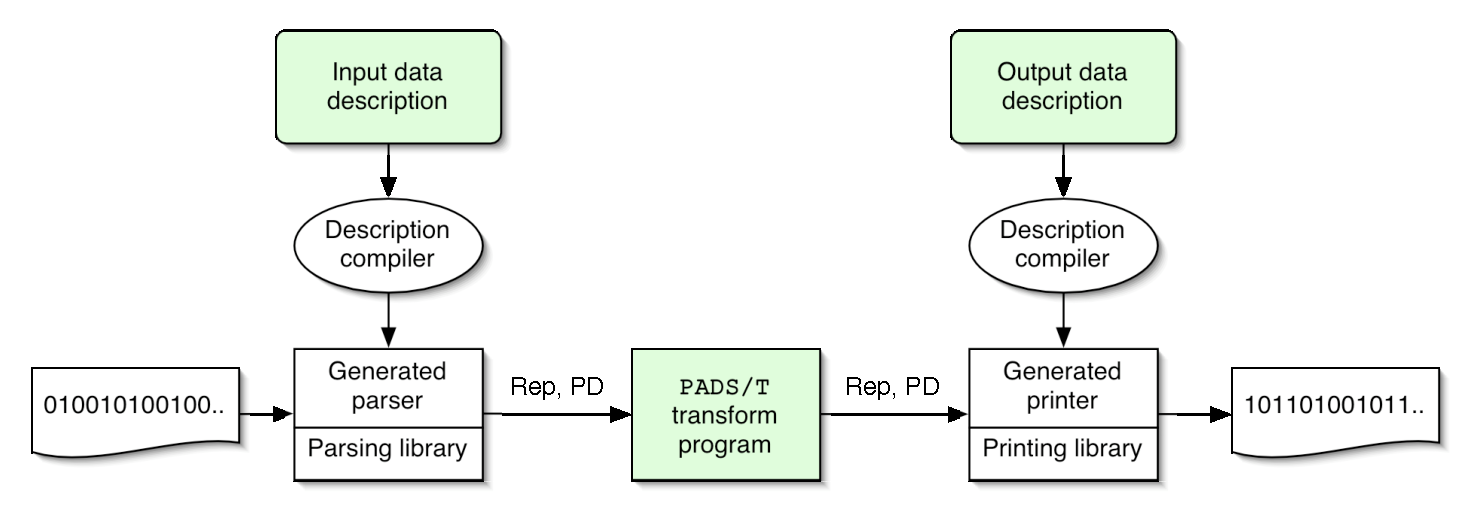
\includegraphics[height=3in,width=5in]{architecture-grant-pads-t}
%  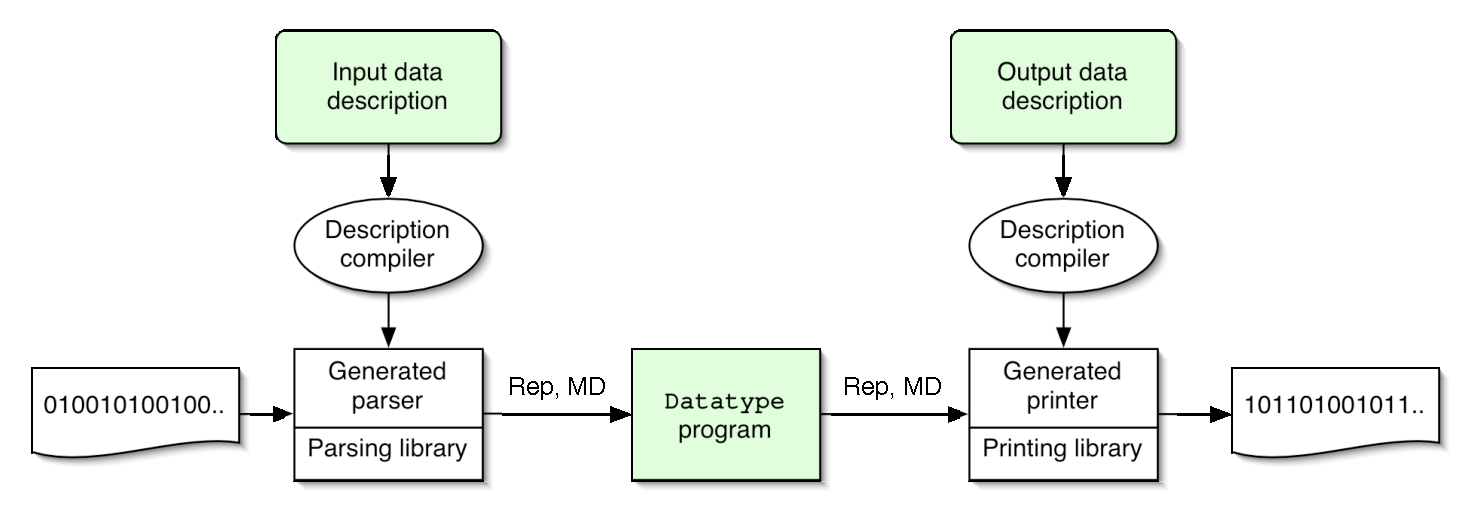
\includegraphics{architecture-grant.eps}
\label{fig:pads-arch}
\caption{Common use of \datatype{} architecture}
\end{figure}

% ---------------------------------------------------

\figref{fig:pads-arch} depicts a common use of the \datatype{}
architecture\footnote{The green boxes denote code written by users.}.
On the upper left, the format of an ad hoc input source is specified
by a user in the \datatype{} data description language.  From this
description, the \datatype{} description compiler produces a custom
parser for instances of the ad hoc input.  Symmetrically, on the
upper-right, the  data description of the output data is compiled into
a custom printer for instances of the ouput.  A \datatype{}
transformation program refers to the types defined by the input and
output descriptions, and the \datatype{} runtime environment for the
transformation program calls the corresponding parsers and printers.

The key abstraction in \datatype{} that supports error-aware computing
is the \emph{\pvalue}, which pairs a data item with its
corresponding meta data.  Meta data includes, among other things,
descriptions of the error content of the data item.  In
\figref{fig:pads-arch}, a \pvalue{} consists of the data item's
\emph{representation} (Rep) and its \emph{parse descriptor} (PD),
which contains the meta data.

\datatype{}'s type system ensures
that data items and their associated meta data are always consistent.
This error-aware computation enables three important language
features:
\begin{enumerate}
\item Safe, error-transparent transformations that need only specify
  how to handle error-free data.
\item Selective querying of errors, which supports easy extraction of detailed error profiles.
\item Flexible, programmatic repair of erroneous, which supports
  disciplined and identifiable correction of errors.
\end{enumerate}


\cut{ - analyst can
  choose when in the processing stream to address errors, rather than
  being forced to drop all faulty records at the beginning of the
  process}

In Section~\ref{sec:data-description}, we introduce \datatype{}'s data
description language using examples from the applications described in
\figref{figure:data-sources} and in
Section~\ref{sec:data-transformation}, we do the same for
\datatype{}'s data-transformation constructs.
Section~\ref{sec:related-work} briefly surveys related work, and in
Section~\ref{sec:conclusion}, we enumerate only a few of the numerous
open problems that await us in \datatype{}'s future.

\cut{ 

INTRO BACK MATTER 

In the next section, we will describe, in detail, the \pads{} approach
to data and meta data (inherited by \datatype{}), the \datatype{}
syntax for data description, and illustrative examples. Next, in
Section~\ref{sec:data-transformation} we will elaborate on
\datatype{}'s support for data transformation, including design,
syntax and some examples.  Section~\ref{sec:related-work} will discuss
the related work. A discussion of conclusions and future work is
included in section~\ref{sec:conclusion}.

% The goal of this paper is to describe a new language for efficient and
% reliable computing with ad hoc data.  More specifically, we describe a
% high-level programming language, \datatype{}, that comes with
% intrinsic support for processing ad hoc data.  Our programming
% language will use the rich data descriptions both as directives for
% parsing ad hoc data sources and as types for describing
% representations of ad hoc data within the programming environment.  In
% addition, a critical facet of our language will be its support for
% {\em error-aware computing}.  Our error-aware infrastructure will
% allow programmers to conveniently verify correctness of data relative
% to a description or alternatively detect data errors and handle them
% in domain-specific ways.  Finally, we will be sure our language design
% is founded on strong programming language principles by studying its
% type system and metatheory extensively.

Solution: Data description Language + transform language
Combine data description language with a transform language.

\pads{} is bound to C. However, functional programming languages are
better suited to the task of data transformation. We therefore propose
a new language, \datatype{}, that combines a data description language
based on the style of ML types (and datatypes) with a functional data
transformation language. 

Our contributions are twofold. First, we propose an ML-style syntax
for the \pads{} data description language, based on type definitions
and {\em(polymorphic coming soon?)} parameterized recursive datatypes
(support for recursive datatypes is new to the \pads{} language, based
on recent results in our other work). This new syntax has a number of
advantages. It is more concise than the C-style encoding and more
naturally suited to describing recursive datatypes. Most importantly,
the new syntax is much more appropriate for transformation language
proposed below, which is based heavily on pattern-matching and data
constructors.

\pads{} provides several data-analysis tools
built upon the generated parsing libraries.

\C{} is a very low-level language that makes transforming ad hoc
data awkward, cumbersome and potentially error-prone.  More
importantly, it provides no intrinsic support for dealing with the
errors that appear in ad hoc data.  In addition, \C's type system and
operational model provide no support for checking the rich invariants
found in ad hoc data either at run time or at compile time.  and
intrinsic mechanisms for checking data invariants at run time

The iterative process of writing a \datatype{} description, parsing ad
hoc data that conforms to that description, and refining the
description results in ``living documentation'' of the data source
that can be in other \datatype{} programs.  

\datatype{} makes it possible to write accurate, complete, and
reusable descriptions of ad hoc data that serve 

Our second contribution is the data transformation language itself.
{\em \pads{} is not a programming language.}  
 
There might be a third:--
collection and analysis a variety of different examples of ad hoc
data from widely differing domains (networking to genomics).  The
analysis of thedifferent sorts of ad hoc data is a substantial
contribution.  It helps usunderstand what is required and what is not.
}